\documentclass[10pt,twocolumn]{article}

\usepackage[margin=0.75in]{geometry}
\usepackage[T1]{fontenc}
\usepackage[utf8]{inputenc}
\usepackage{times}
\usepackage{graphicx}
\usepackage{subcaption}
\usepackage{booktabs}
\usepackage{multirow}
\usepackage{array}
\usepackage{hyperref}
\usepackage{url}
\usepackage{enumitem}

\hypersetup{
  colorlinks=true,
  linkcolor=blue,
  citecolor=blue,
  urlcolor=blue
}

\title{LoRA-Adapted RETFound with Multi-Scale Fusion and Ordinal Losses\\for Five-Class Diabetic Retinopathy Grading and External Validation}
\author{
Nilotpal Bose\\
Department of Computer Science and Engineering\\
\texttt{[update-email]}
}
\date{}

\begin{document}
\maketitle

\begin{abstract}
Adapting retinal foundation models for ordered DR severity remains challenging when flat cross-entropy ignores class imbalance and clinical ordinal structure. We compare RETFound Baseline (full fine-tuning with weighted cross-entropy) and Enhanced RETFound (LoRA adapters, multi-scale token fusion, and focal/ordinal/referable losses) for five-class diabetic retinopathy grading. On APTOS 2019 (test N = 550), Enhanced RETFound slightly improved quadratic weighted kappa (QWK 0.893 vs 0.888) and referable AUROC (0.987 vs 0.981), while the baseline retained higher accuracy (0.831 vs 0.811). On external Messidor-2 without fine-tuning, Enhanced RETFound improved QWK (0.505 vs 0.488) and referable AUROC (0.778 vs 0.725). Ablations show A2 (LoRA + multi-scale + focal) achieves the best APTOS QWK (0.895), whereas ordinal/referable auxiliaries mainly boost screening AUROC. Overall, Enhanced RETFound is comparable in-domain and stronger under external shift for ordinal and screening-oriented metrics.
\end{abstract}

\noindent\textbf{Index Terms:} diabetic retinopathy, RETFound, foundation model, LoRA, ordinal regression, QWK, external validation.

\section{Introduction}
Diabetic retinopathy is a microvascular complication of diabetes and a major cause of preventable vision loss worldwide. Population screening relies on grading colour fundus photographs according to clinical severity scales such as ICDR (grade 0 to grade 4). Because grading is labour-intensive and subject to inter-observer variability, deep learning has been widely explored for automated DR detection and staging.

Early systems were typically trained from scratch or from ImageNet-initialised convolutional networks on large labelled fundus corpora. More recently, foundation models pretrained with self-supervised learning on massive unlabelled medical image collections have emerged as a stronger starting point for downstream clinical tasks. RETFound is a retinal foundation model based on a Vision Transformer pretrained with masked autoencoding on approximately 1.6 million fundus and OCT images.

Despite this progress, adapting RETFound to DR severity grading still raises open questions. Standard full fine-tuning with flat cross-entropy treats grades as unordered classes and may under-emphasise rare mild/severe cases and ordinal structure. Parameter-efficient fine-tuning methods such as LoRA, multi-scale feature aggregation, and imbalance-/ordinal-aware losses offer a more clinically aligned adaptation recipe.

\section{Materials and Methods}
\subsection{Dataset Description}
APTOS 2019 Blindness Detection provides labelled macular-centred fundus photographs with ICDR-aligned grades 0--4. We used a stratified 70/15/15 train/validation/test split fixed in \texttt{splits.json} (test N = 550). Images were resized to $224\times224$, normalised with ImageNet statistics, and lightly augmented.

Messidor-2 is used strictly as an external test set (no fine-tuning). We report both five-class grading and referable DR (grade $\geq$ 2).

\subsection{Frameworks for Comparison}
Two frameworks share the same RETFound ViT-Large/16 colour-fundus pretrained backbone and the same preprocessing.
\begin{itemize}[leftmargin=*,noitemsep,topsep=2pt]
  \item \textbf{RETFound Baseline:} full encoder fine-tuning + weighted cross-entropy.
  \item \textbf{Enhanced RETFound:} frozen backbone with LoRA adapters on attention \texttt{qkv} (~1.3\% trainable parameters), multi-depth feature fusion (blocks 7, 15, 23), and focal + CORAL ordinal + referable auxiliary losses.
\end{itemize}

We also evaluate three 15-epoch ablations: A1 (LoRA + late + focal), A2 (A1 + multi-scale), A3 (A2 + ordinal/referable auxiliaries).

\subsection{Metrics}
We report accuracy, macro-F1, QWK, referable accuracy/AUROC, confusion matrices, and ROC curves. Primary interpretation emphasises QWK and referable AUROC.

\section{Results}
\subsection{Main Comparison on APTOS and Messidor-2}
\begin{table}[t]
\centering
\caption{Main results (checkpoints selected by best validation QWK).}
\label{tab:main}
\scriptsize
\setlength{\tabcolsep}{3pt}
\begin{tabular}{l l c c c c c}
\toprule
Model & Set & Acc & M-F1 & QWK & R-Acc & R-AUC \\
\midrule
Baseline & APTOS & 0.831 & 0.671 & 0.888 & 0.929 & 0.981 \\
Enhanced & APTOS & 0.811 & 0.683 & 0.893 & 0.935 & 0.987 \\
Baseline & Messidor-2 & 0.612 & 0.330 & 0.488 & 0.807 & 0.725 \\
Enhanced & Messidor-2 & 0.593 & 0.349 & 0.505 & 0.802 & 0.778 \\
\bottomrule
\end{tabular}
\end{table}

Enhanced RETFound yields a small in-domain gain in QWK (+0.005) and referable AUROC (+0.006), while Baseline remains higher in overall accuracy (+0.020). Externally, Enhanced improves QWK (+0.017) and referable AUROC (+0.053), indicating stronger robustness for clinically relevant endpoints.

\begin{figure}[t]
\centering
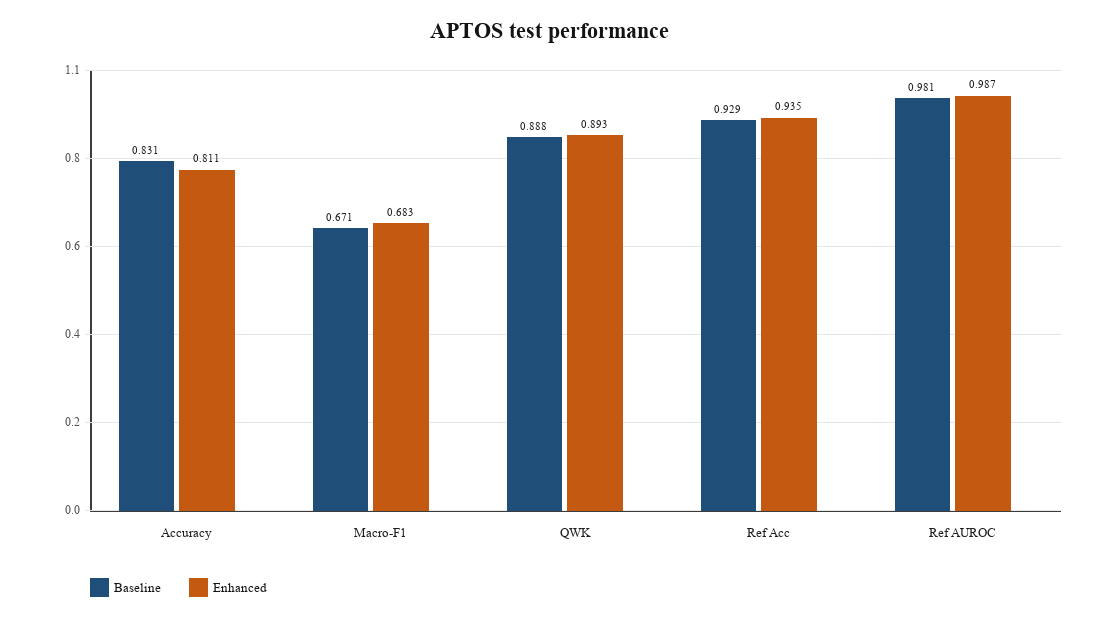
\includegraphics[width=\columnwidth]{../figures/fig1_aptos_comparison.png}
\caption{APTOS test metrics for RETFound Baseline versus Enhanced RETFound.}
\label{fig:aptos-bars}
\end{figure}

\begin{figure}[t]
\centering
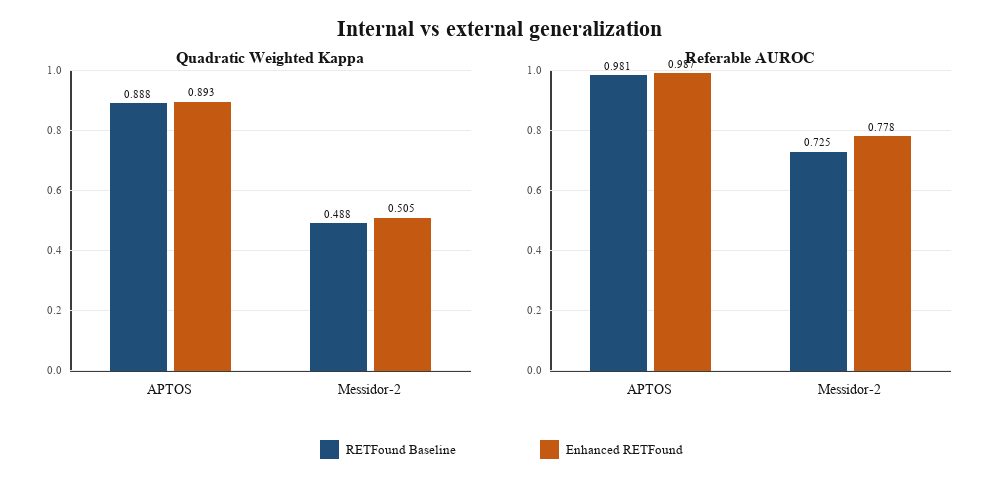
\includegraphics[width=\columnwidth]{../figures/fig3_internal_vs_external.png}
\caption{Internal (APTOS) vs external (Messidor-2) QWK and referable AUROC.}
\label{fig:internal-external}
\end{figure}

\subsection{Validation QWK Curves}
\begin{figure}[t]
\centering
\begin{subfigure}[t]{0.49\columnwidth}
  \centering
  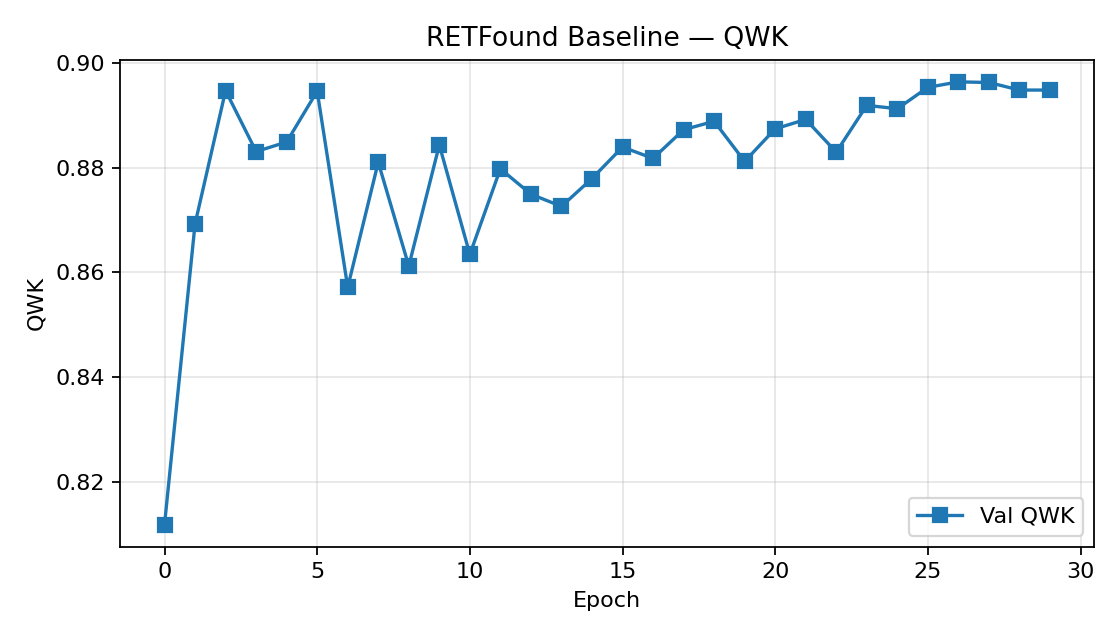
\includegraphics[width=\linewidth]{../figures/main_baseline_qwk.png}
  \caption{Baseline}
\end{subfigure}
\hfill
\begin{subfigure}[t]{0.49\columnwidth}
  \centering
  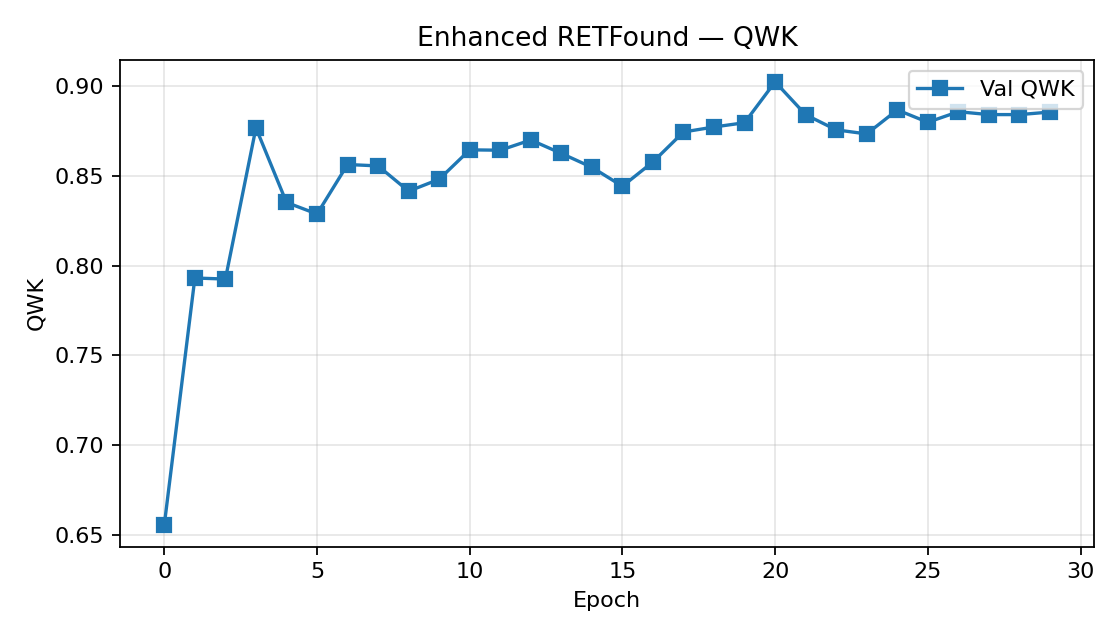
\includegraphics[width=\linewidth]{../figures/main_enhanced_qwk.png}
  \caption{Enhanced}
\end{subfigure}
\caption{Validation QWK for main models.}
\label{fig:main-qwk}
\end{figure}

\begin{figure}[t]
\centering
\begin{subfigure}[t]{0.32\columnwidth}
  \centering
  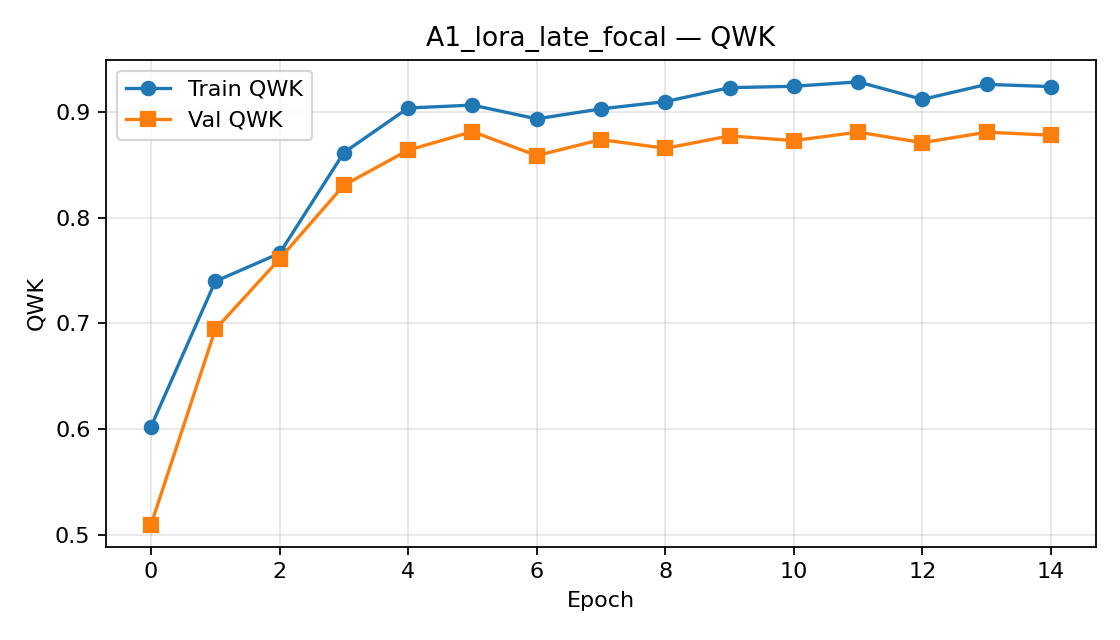
\includegraphics[width=\linewidth]{../figures/ablation_A1_lora_late_focal_qwk.png}
  \caption{A1}
\end{subfigure}
\hfill
\begin{subfigure}[t]{0.32\columnwidth}
  \centering
  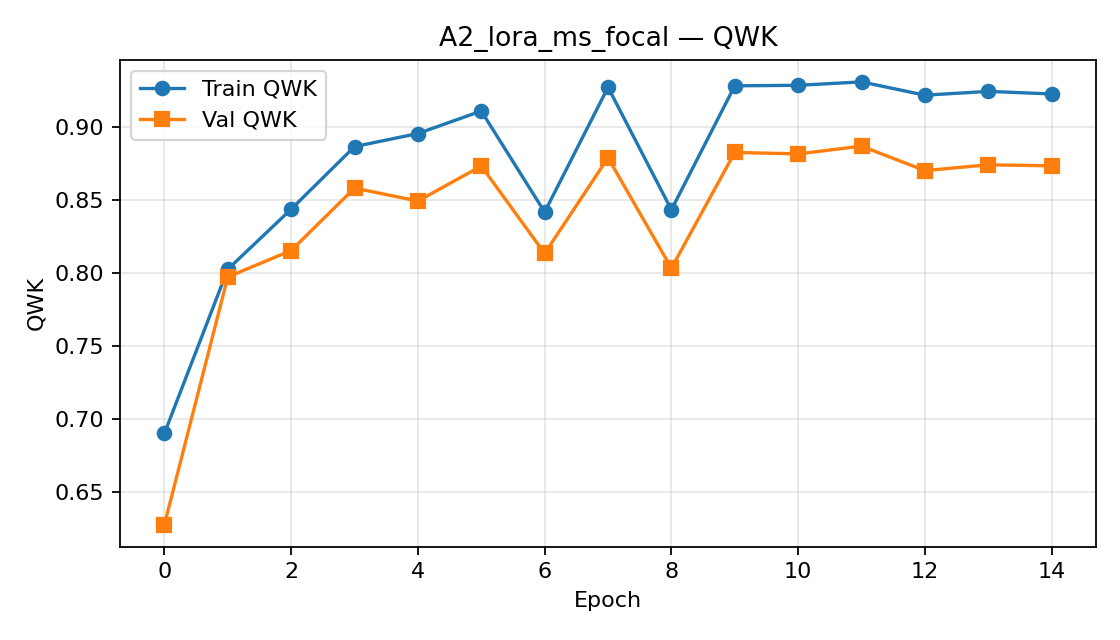
\includegraphics[width=\linewidth]{../figures/ablation_A2_lora_ms_focal_qwk.png}
  \caption{A2}
\end{subfigure}
\hfill
\begin{subfigure}[t]{0.32\columnwidth}
  \centering
  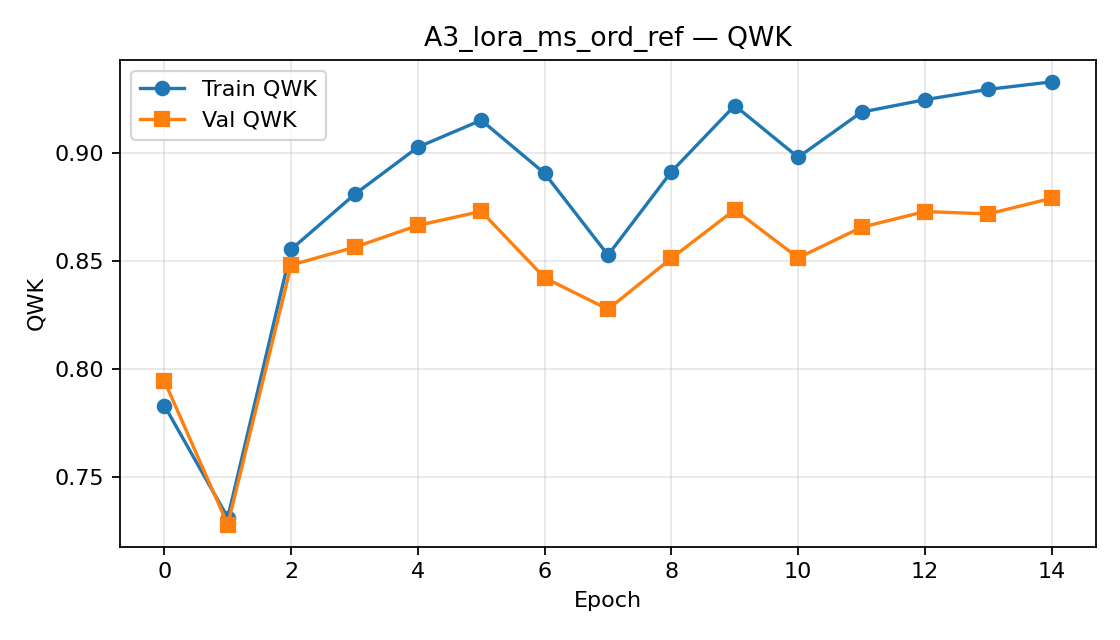
\includegraphics[width=\linewidth]{../figures/ablation_A3_lora_ms_ord_ref_qwk.png}
  \caption{A3}
\end{subfigure}
\caption{Validation QWK for ablations (15 epochs).}
\label{fig:ablation-qwk}
\end{figure}

\subsection{External Validation and Error Structure}
\begin{figure}[t]
\centering
\begin{subfigure}[t]{0.49\columnwidth}
  \centering
  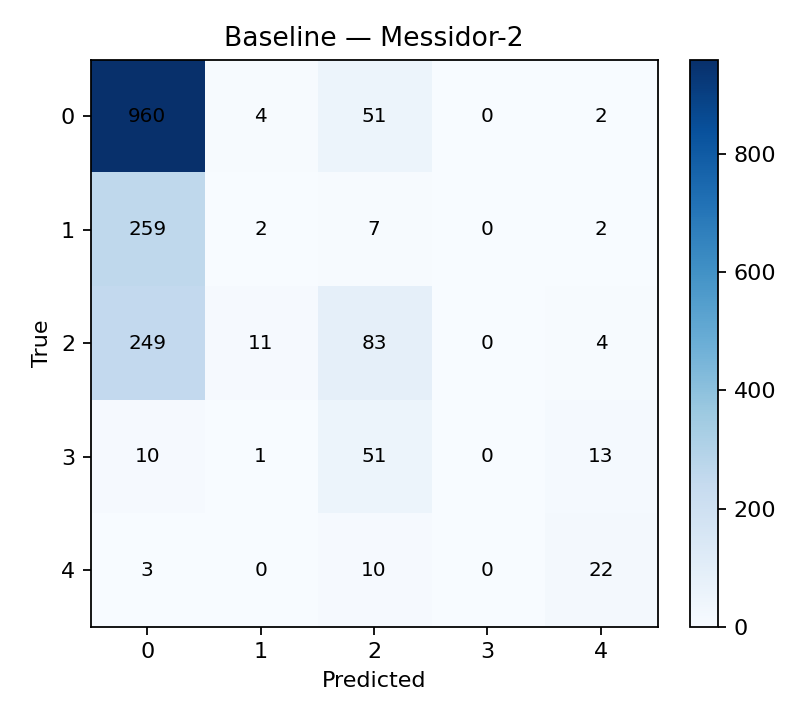
\includegraphics[width=\linewidth]{../figures/cm_baseline_external.png}
  \caption{Baseline external CM}
\end{subfigure}
\hfill
\begin{subfigure}[t]{0.49\columnwidth}
  \centering
  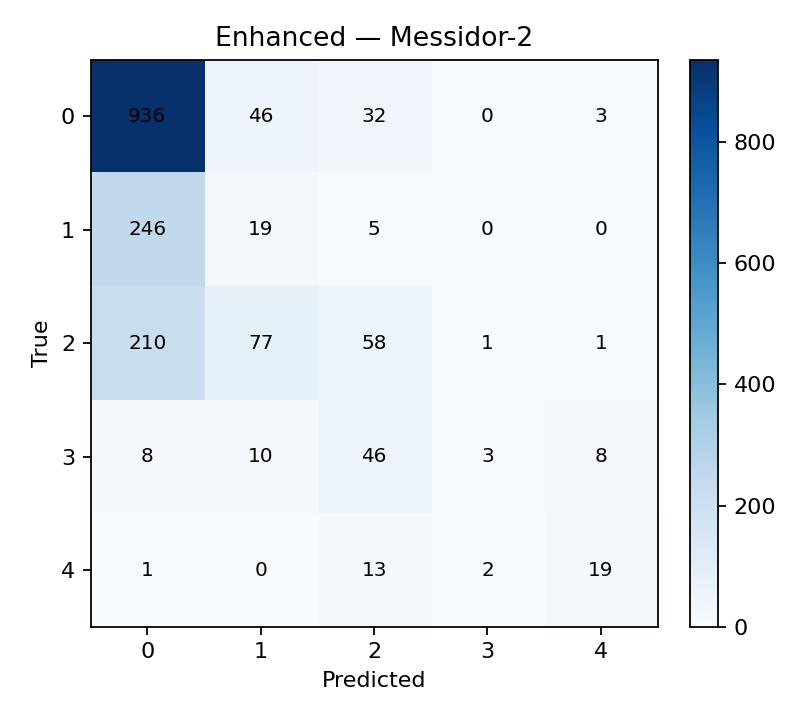
\includegraphics[width=\linewidth]{../figures/cm_enhanced_external.png}
  \caption{Enhanced external CM}
\end{subfigure}
\caption{Messidor-2 confusion matrices.}
\label{fig:external-cm}
\end{figure}

\begin{figure}[t]
\centering
\begin{subfigure}[t]{0.49\columnwidth}
  \centering
  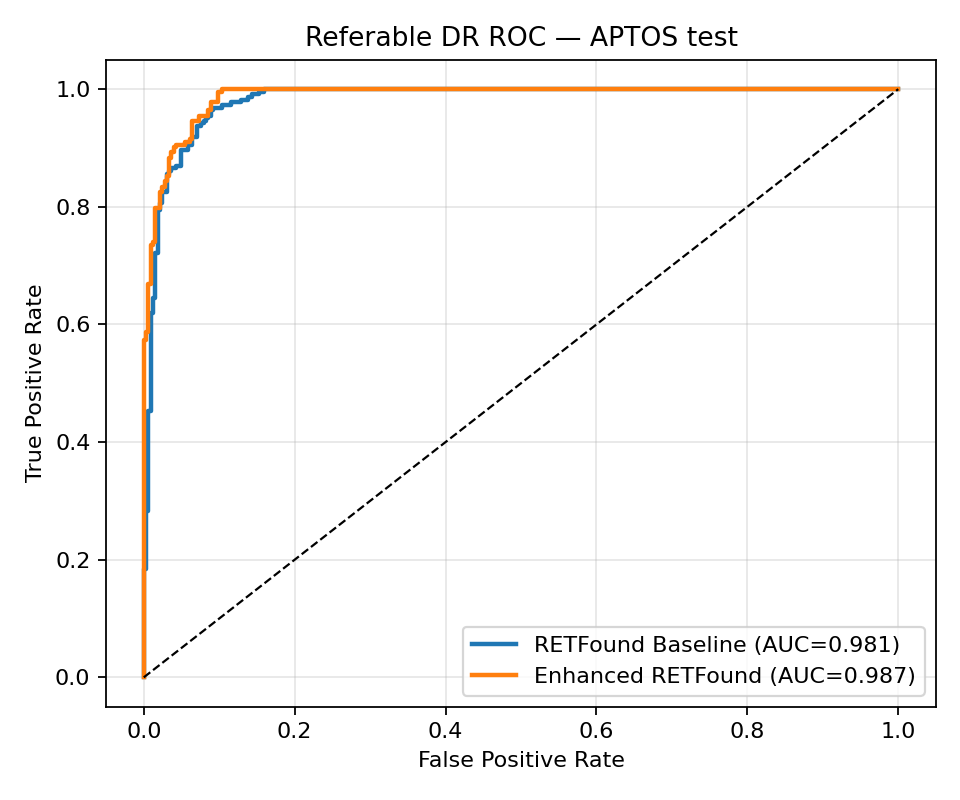
\includegraphics[width=\linewidth]{../figures/roc_referable_aptos.png}
  \caption{APTOS referable ROC}
\end{subfigure}
\hfill
\begin{subfigure}[t]{0.49\columnwidth}
  \centering
  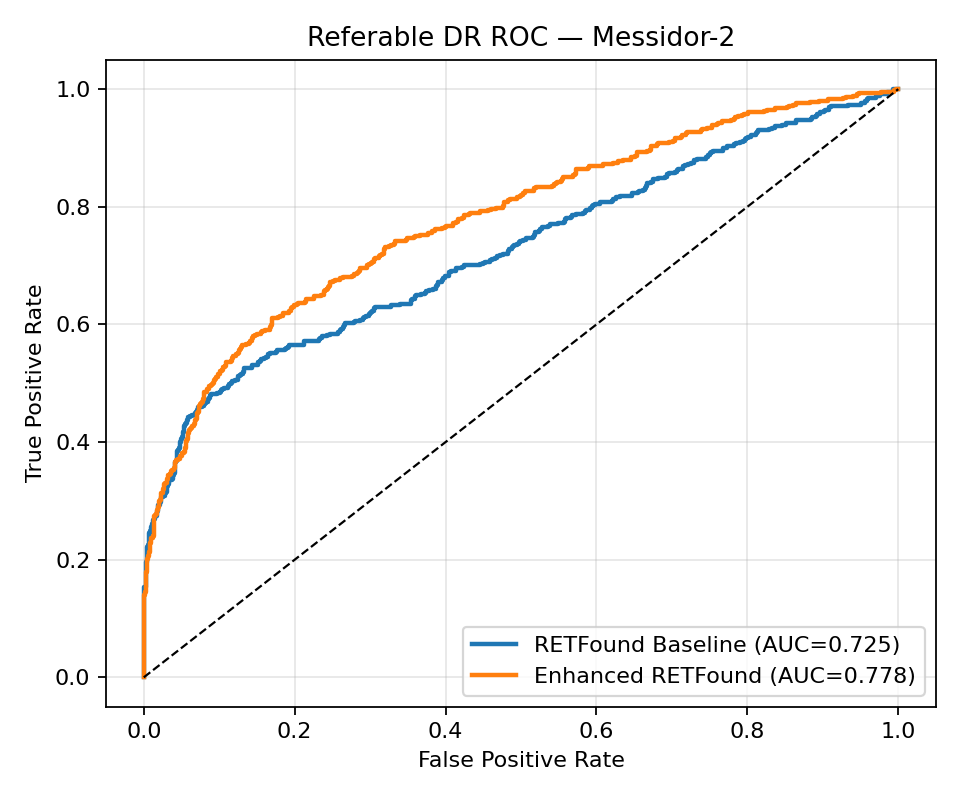
\includegraphics[width=\linewidth]{../figures/roc_referable_external.png}
  \caption{Messidor-2 referable ROC}
\end{subfigure}
\caption{Referable DR ROC comparison.}
\label{fig:referable-roc}
\end{figure}

\subsection{APTOS Confusion Matrices and Ablations}
\begin{figure}[t]
\centering
\begin{subfigure}[t]{0.49\columnwidth}
  \centering
  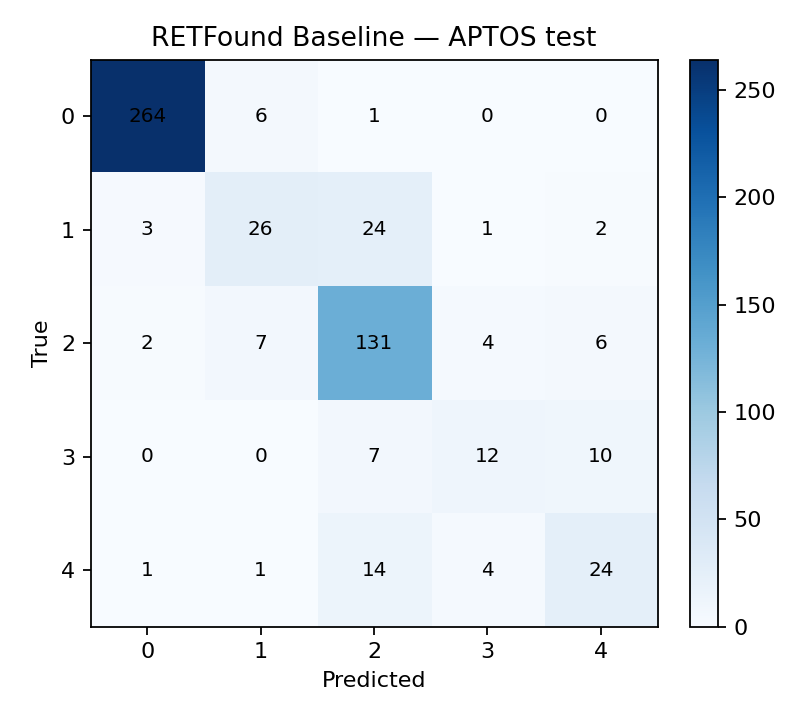
\includegraphics[width=\linewidth]{../figures/cm_baseline_aptos.png}
  \caption{Baseline APTOS CM}
\end{subfigure}
\hfill
\begin{subfigure}[t]{0.49\columnwidth}
  \centering
  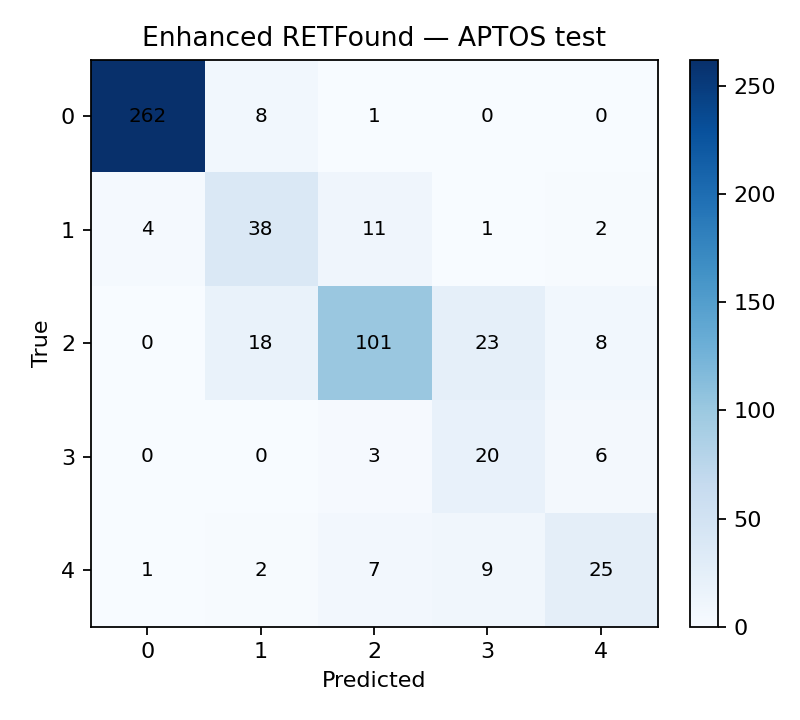
\includegraphics[width=\linewidth]{../figures/cm_enhanced_aptos.png}
  \caption{Enhanced APTOS CM}
\end{subfigure}
\caption{APTOS confusion matrices.}
\label{fig:aptos-cm}
\end{figure}

\begin{table}[t]
\centering
\caption{Ablation results on APTOS (15 epochs; best validation-QWK checkpoint).}
\label{tab:ablation}
\scriptsize
\setlength{\tabcolsep}{3pt}
\begin{tabular}{l c c c}
\toprule
Variant & Acc & QWK & Ref-AUC \\
\midrule
Baseline & 0.831 & 0.888 & 0.981 \\
Enhanced & 0.811 & 0.893 & 0.987 \\
A1 & 0.738 & 0.892 & 0.985 \\
A2 & 0.765 & \textbf{0.895} & 0.987 \\
A3 & 0.764 & 0.881 & \textbf{0.988} \\
\bottomrule
\end{tabular}
\end{table}

\begin{figure}[t]
\centering
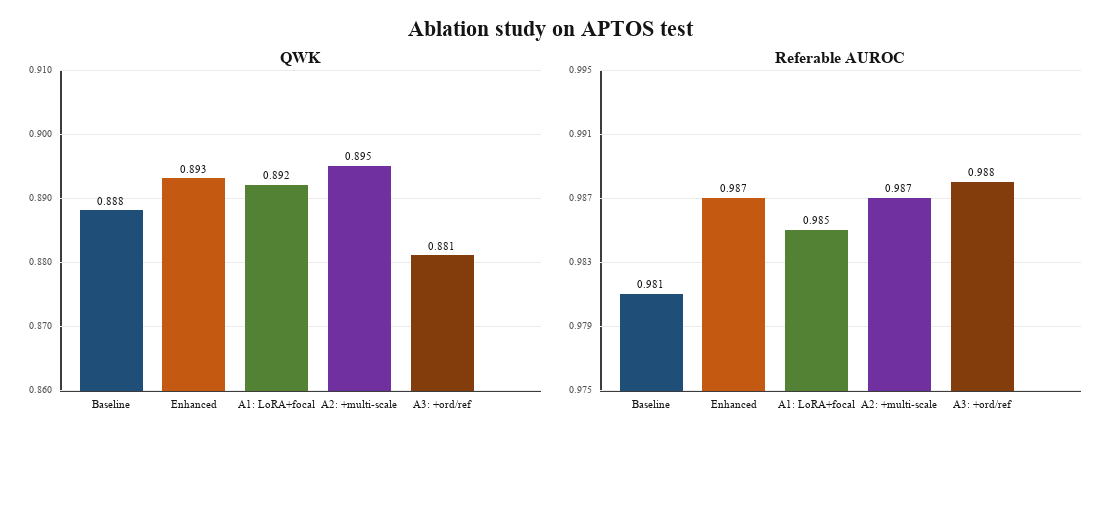
\includegraphics[width=\columnwidth]{../figures/fig4_ablation_qwk_auroc.png}
\caption{Ablation summary on APTOS: QWK and referable AUROC.}
\label{fig:ablation-summary}
\end{figure}

\section{Discussion}
The results suggest metric-dependent trade-offs. For strict five-class ordinal agreement, A2 (LoRA + multi-scale + focal) performs best. For screening-focused use, auxiliary objectives improve referable AUROC, especially under external shift.

\section{Conclusion}
Enhanced RETFound is comparable to full fine-tuning in-domain and stronger externally on ordinal/screening metrics. Foundation-model adaptation for DR should be assessed with clinically meaningful endpoints and external validation, not accuracy alone.

\section*{References}
\begin{enumerate}\itemsep0pt
  \item Y. Zhou et al., ``A foundation model for generalizable disease detection from retinal images,'' \textit{Nature}, 2023.
  \item A. Dosovitskiy et al., ``An image is worth 16x16 words,'' \textit{ICLR}, 2021.
  \item K. He et al., ``Masked autoencoders are scalable vision learners,'' \textit{CVPR}, 2022.
  \item E. J. Hu et al., ``LoRA: Low-rank adaptation of large language models,'' \textit{ICLR}, 2022.
  \item T.-Y. Lin et al., ``Focal loss for dense object detection,'' \textit{ICCV}, 2017.
  \item W. Cao et al., ``Rank consistent ordinal regression for neural networks,'' \textit{Pattern Recognit. Lett.}, 2020.
  \item C. P. Wilkinson et al., ``Proposed international clinical DR severity scales,'' \textit{Ophthalmology}, 2003.
  \item V. Gulshan et al., ``Development and validation of a deep learning algorithm for DR detection,'' \textit{JAMA}, 2016.
  \item E. Decenci\`ere et al., ``Feedback on a publicly distributed image database: the Messidor database,'' \textit{Image Anal. Stereol.}, 2014.
  \item APTOS 2019 Blindness Detection, Kaggle: \url{https://www.kaggle.com/competitions/aptos2019-blindness-detection}.
  \item J. Krause et al., ``Grader variability and reference standards for DR ML evaluation,'' \textit{Ophthalmology}, 2018.
  \item D. S. W. Ting et al., ``Artificial intelligence and deep learning in ophthalmology,'' \textit{Br. J. Ophthalmol.}, 2019.
  \item T. Li et al., ``Diagnostic assessment of deep learning algorithms for DR screening,'' \textit{Inf. Sci.}, 2019.
  \item J. Cohen, ``Weighted kappa,'' \textit{Psychol. Bull.}, 1968.
  \item R. Bommasani et al., ``On the opportunities and risks of foundation models,'' \textit{arXiv:2108.07258}, 2021.
\end{enumerate}

\end{document}

